\chapter{Finite automata minimization algorithms}

\section{Introduction}

\section{Brzozowski's algorithm}

\begin{flushleft}
$\epsilon-free$ FA: $M_0=(Q_0,V,T_0,\emptyset,S_0,F_0)$ \\
to be minimized $DFA$: $M_2=(Q_2,V,T_2,\emptyset,S_2,F_2)$ \\
intermediate $NFA$: $M_1=(Q_1,V,T_1,\emptyset,S_1,F_1)$\\
\end{flushleft}

NFA: $M_1 \to $ DFA: $M_2, M_2=suseful_s\circ subsetopt(M_1)$
\begin{align*}
& q_0,q_1\in Q_1,Q_2\subseteq\mathbb{P}(Q_1),\forall p\in  Q_2,p=(q_0,q_1)\\
& \overrightarrow{L}_{M_2}(p)=\overrightarrow{L}_{M_1}(q_0)\cup  \overrightarrow{L}_{M_1}(q_1)\\
& \Rightarrow \\
& \overrightarrow{L}_{M_2}(p)=\bigcup_{q\in p}\overrightarrow{L}_{M_1}(q)\\
& \Rightarrow 
\end{align*}

\begin{figure}[htbp]
	\begin{tikzpicture}
	\matrix (a) [matrix of math nodes,row sep=3em,
	column sep=5em, nodes in empty cells]
	{ Q_1 &  P(Q_1) \\ 
		&  D(Q_2) \\};
	\path[>=latex,->] 
	(a-1-1) edge node [auto] {$subsetopt$} (a-1-2)
	edge node [auto,swap] {$$} (a-2-2)
	(a-1-2) edge node [auto] {$useful_s$} (a-2-2)
	;
	\end{tikzpicture}
	\caption{$M_2=suseful_s\circ subsetopt(M_1)$}
\end{figure}

\begin{figure}[htbp]
	\subfigure[$M_1=(Q_1,V,T_1,\emptyset,S_1,F_1)$] { \label{fig:a} 
	\begin{tikzpicture}[->,>=stealth',shorten >=1pt,auto,node distance=2cm, semithick]
		\tikzstyle{every state}=[minimum size=0.1mm]
		\node[state] (q)  [] {$q$};
		\node[state] (q0) [above right of=q] {$q_0$};
		\node[state] (q1) [below right of=q] {$q_1$};
		\node[state] (f1)  [below right of=q0] {$f_1$};
		\path 
		(q) edge [] node {$a$} (q0)
		    edge [swap] node {$a$} (q1)
		(q0) edge [] node {$\overrightarrow{L}_{M_1}(q_0)$} (f1)
		(q1) edge [swap] node {$\overrightarrow{L}_{M_1}(q_1)$} (f1)
		;
	\end{tikzpicture}
    }
    \hspace{2cm}
	\subfigure[$M_2=(Q_2,V,T_2,\emptyset,S_2,F_2)$] { \label{fig:b}
    \begin{tikzpicture}[->,>=stealth',shorten >=1pt,auto,node distance=3cm, semithick,scale=4]
    	\tikzstyle{every state}=[minimum size=0.1mm]
    	\node[state] (q01)  {$(q_0,q_1)$};
    	\node[state] (f2)  [right of=q01] {$f_2$};
    	\path 
    	(q01) edge [bend left] node {$\overrightarrow{L}_{M_1}(q_0)$} (f2)
    	(q01) edge [bend right,swap] node {$\overrightarrow{L}_{M_1}(q_1)$} (f2)
    	;
    \end{tikzpicture}
    }
	\caption{$M_2=suseful_s\circ subsetopt(M_1)$}
\end{figure}

\begin{figure}[htbp]
	\subfigure[$M_0=(Q_0,V,T_0,\emptyset,S_0,F_0)$] {
		\begin{tikzpicture}[->,>=stealth',shorten >=1pt,auto,node distance=2cm, semithick]
		\tikzstyle{every state}=[minimum size=0.1mm]
		\node[state,accepting] (q2) []{$q_2$};
		\node[state,initial] (q0) [above left of=q2] {$q_0$};
		\node[state] (q1) [above right of=q2] {$q_1$};
		\path
		(q0) edge[bend left] node {$0$} (q1)
		(q1) edge[bend left] node {$0$} (q0)
		(q0) edge[swap] node {$1$} (q2)
		(q1) edge[] node {$1$} (q2)
		(q2) edge[loop below] node {$0,1$} (q2)
		;
		\end{tikzpicture}
	}
    \hspace{1cm}
	\subfigure[$M^R_0=(Q_0,V,T_0,\emptyset,S_0,F_0)^R=(Q_0,V,T^R,\emptyset,F_0,S_0)$]{
		\begin{tikzpicture}[->,>=stealth',shorten >=1pt,auto,node distance=2cm, semithick]
		\tikzstyle{every state}=[minimum size=0.1mm]
		\node[state,initial] (q2) []{$q_2$};
		\node[state,accepting] (q0) [above left of=q2] {$q_0$};
		\node[state] (q1) [above right of=q2] {$q_1$};
		\path
		(q1) edge[bend right,swap] node {$0$} (q0)
		(q0) edge[bend right,swap] node {$0$} (q1)
		(q2) edge[] node {$1$} (q0)
		(q2) edge[swap] node {$1$} (q1)
		(q2) edge[loop below] node {$0,1$} (q2)
		;
		\end{tikzpicture}
	}
    \newline
	\subfigure[$useful_s\circ subsetopt\circ R(M_0)$]{
		\begin{tikzpicture}[->,>=stealth',shorten >=1pt,auto,node distance=2cm, semithick]
		\tikzstyle{every state}=[minimum size=0.1mm]
		\node[state,initial] (q2) []{$q_2$};
		\node[state,accepting] (q0) [above of=q2] {$\{q_0,q_1,q_2\}$};
		\path
		(q2) edge[] node {$1$} (q0)
		(q0) edge[loop above] node {$0,1$} (q0)
		(q2) edge[loop below] node {$0$} (q2)
		;
	\end{tikzpicture}
	}
    \hspace{3cm}
    \subfigure[$M_1=R\circ useful_s\circ subsetopt\circ R(M_0)$]{
    	\begin{tikzpicture}[->,>=stealth',shorten >=1pt,auto,node distance=2cm, semithick]
    	\tikzstyle{every state}=[minimum size=0.1mm]
    	\node[state,accepting] (q2) []{$q_2$};
    	\node[state,initial] (q0) [above of=q2] {$\{q_0,q_1,q_2\}$};
    	\path
    	(q0) edge[] node {$1$} (q2)
    	(q0) edge[loop above] node {$0,1$} (q0)
    	(q2) edge[loop below] node {$0$} (q2)
    	;
    	\end{tikzpicture}
    }
    \caption{$M_1=R\circ useful_s\circ subsetopt\circ R(M_0)$}
\end{figure}

\begin{figure}[htbp]
	\begin{align*}
	\text{start: } &U=\{q_2\}\\
	u=q_2: & T(q_2,0)=\{q_2\},T(q_2,1)=\{q_0,q_1,q_2\} \\
	&\text{add new start to $D$, } D=\{q_2,\{q_0,q_1,q_2\}\} \\
	u=\{q_0,q_1,q_2\}:& T(\{q_0,q_1,q_2\},0)=T(q_0,0)\cup T(q_1,0)\cup T(q_2,0)=\{q_1\}\cup \{q_0\}\cup \{q_2\} =\{q_0,q_1,q_2\}\\
	&T(\{q_0,q_1,q_2\},1)=T(q_0,1)\cup T(q_1,1)\cup T(q_2,1)=\emptyset\cup \emptyset \cup \{q_0,q_1,q_2\}=\{q_0,q_1,q_2\}
	\end{align*}
	
	\subfigure[$M$]{
		\begin{tikzpicture}[->,>=stealth',shorten >=1pt,auto,node distance=2cm, semithick]
		\tikzstyle{every state}=[minimum size=0.1mm]
		\node[state,initial] (q2) []{$q_2$};
		\node[state,accepting] (q0) [above left of=q2] {$q_0$};
		\node[state] (q1) [above right of=q2] {$q_1$};
		\path
		(q1) edge[bend right,swap] node {$0$} (q0)
		(q0) edge[bend right,swap] node {$0$} (q1)
		(q2) edge[] node {$1$} (q0)
		(q2) edge[swap] node {$1$} (q1)
		(q2) edge[loop below] node {$0,1$} (q2)
		;
		\end{tikzpicture}
	}
    \hspace{2cm}
	\subfigure[$useful_s\circ subsetopt(M)$]{
		\begin{tikzpicture}[->,>=stealth',shorten >=1pt,auto,node distance=2cm, semithick]
		\tikzstyle{every state}=[minimum size=0.1mm]
		\node[state,initial] (q2) []{$q_2$};
		\node[state,accepting] (q0) [right of=q2] {$\{q_0,q_1,q_2\}$};
		\path
		(q2) edge[] node {$1$} (q0)
		(q0) edge[loop above] node {$0,1$} (q0)
		(q2) edge[loop above] node {$0$} (q2)
		;
		\end{tikzpicture}
	}
	\caption{$useful_s\circ subsetopt(M)$}
\end{figure}

\section{Minimization by equivalence of states}

\begin{figure}[htbp]
	Equivalence relation $E\subseteq Q\times Q$\\
	$(p,q)\in E\equiv (\overrightarrow{L}(p)=\overrightarrow{L}(q))$\\
	
	\subfigure[$(p,q)\in E$]{
		\begin{tikzpicture}[->,>=stealth',shorten >=1pt,auto,node distance=2cm, semithick]
		\tikzstyle{every state}=[minimum size=0.1mm]
		\node[state,accepting] (f) {$f$};
		\node[state] (p) [above left of=f]{$p$};
		\node[state] (q) [below left of=f]{$q$};
		\path
		(p) edge[] node {$\overrightarrow{L}(p)$} (f)
		(q) edge[swap] node {$\overrightarrow{L}(q)$} (f)
		;
		\end{tikzpicture}
		}
	    \hspace{2cm}
    	\subfigure[$(p,q)\in E$]{
    	\begin{tikzpicture}[->,>=stealth',shorten >=1pt,auto,node distance=2cm, semithick]
    	\tikzstyle{every state}=[minimum size=0.1mm]
    	\node[state,accepting] (f) {$f$};
    	\node[state] (p) [left of=f]{$[p,q]$};
    	\path
    	(p) edge[] node {$\overrightarrow{L}(\#)$} (f)
    	;
    	\end{tikzpicture}
   		}
	\caption{Equivalence relation $E\subseteq Q\times Q$}
\end{figure}

\begin{figure}[htbp]
	$\overrightarrow{L}(p)=\bigcup_{a\in V}(\{a\} \cdot \overrightarrow{L}(T(p,a)) \cup \{\epsilon|p\in F\}$\\

	\begin{tikzpicture}[->,>=stealth',shorten >=1pt,auto,node distance=3cm, semithick]
		\tikzstyle{every state}=[minimum size=0.1mm]
		\node[state,accepting] (p) {$p$};
		\node[state] (q1) [above right of=p]{$T(p,a)$};
		\node[state] (q2) [below right of=p]{$T(p,b)$};
		\node[state,accepting] (f1) [right of=q1]{$f1$};
		\node[state,accepting] (f2) [right of=q2]{$f2$};
		\path
		(p) edge[] node {$a$} (q1)
		(p) edge[] node {$b$} (q2)
		(q1) edge[] node {$\overrightarrow{L}(T(p,a))$} (f1)
		(q2) edge[] node {$\overrightarrow{L}(T(p,b))$} (f2)
		;
	\end{tikzpicture}
	\caption{$L(p)$}
\end{figure}

Let $A=(Q,V,T,_,F)$ be a deterministic finite automaton, where $Q$ is a finite set of states, $V$ is a finite set of input symbols, $T$ is a mapping from $Q\times V$ into $Q$, and $F\subseteq Q$ is the set of final states. No initial state is specified since it is of no importance in what follows. The mapping $T$ is extended to $T\times V^\ast$ in the usual manner where $V^\ast$ denotes the set of all finite strings (including the empty string $\epsilon$) of symbols from $V$

\begin{definition}[equivalent states]
	The states $s$ and $t$ are said to be equivalent if for each $x\in V^\ast, T(s,x)\in F$ if and only if $T(t,x)\in F$. 
\end{definition}

\section{From \cite{Hopcroft71}}

The algorithm for finding the equivalence classes of Q is described below:

\begin{algorithm}  
	\caption{The algorithm for finding the equivalence classes of Q}  
	\begin{algorithmic}%[1] %每行显示行号  
		\Require $M=(Q,V,T,\_,F)$  
		\Ensure The equivalence classes of $Q$  
		\State Step 1. For each $s\in Q$ and each $a\in V$ construct
		
		$T^{-1}(s,a)=\{t|T(t,a)=s\}$ \qquad 计算状态s的in-transitionsss
		
		\State Step 2. construct $B(1)=F, B(2)=Q-F$ and for each $a\in V$ and $1\le i\le 2$ construct
		
		\For{each $a\in V$ }
			\For{$i=1$; $i<n$; $i++$ }  
				\State $\hat{B}(B(i),a)=\{s|s\in B(i) \text{ and } T^{-1}(s,a)\ne \emptyset\}$;
			\EndFor  
		\EndFor 
		\State Step 3. Set $k=3$;
		\State Step 4. For each $a\in V$ construct $L(a)$
		\For{each $a\in V$ }
			\If {$|\hat{B}(B(1),a)| \le |\hat{B}(B(2),a)|$}
				\State $L(a) = \hat{B}(B(1),a)$;
			\Else
	            \State $L(a) = \hat{B}(B(2),a)$; 
			\EndIf
		\EndFor
		\State Step 5. Select $a\in V$ and $i\in L(a)$. The algorithm terminates when $L(a)=\emptyset$ for each $a\in V$.
		\State Step 6. Delete $i$ from $L(a)$.
		\State Step 7. For each $j<k$ such that there exists $t\in B(j)$ with $T(t,a)\in \hat{B}(B(i),a)$, perform steps 7a,7b,7c, and 7d.
		
		\State Step 7a. partition $B(j)$ into
			
			$B^\prime(j)=\{t|T(t,a)\in \hat{B}(B(i),a)\}$ and			
		
			$B^{\prime\prime}(j)=B(j)-B^\prime(j)$
		
		\State Step 7b. Replace $B(j)$ by $B^\prime(j)$ and constant $B(k)=B^{\prime\prime}$. Construct the corresponding $\hat{B}(B(j),a)$ and $\hat{B}(B(k),a)$ for each $a\in V$.
		
		\State Step 7c. For each $a\in V$ modify $L(a)$ as follows.
			\If{$j\notin L(a) \& 0<|\hat{B}(B(j),a)|\le |\hat{B}(B(k)),a|$}
				\State $L(a) = L(a)\cup \{j\}$;
			\Else
				\State $L(a) = L(a)\cup \{k\}$;
			\EndIf 
			
		\State Step 7d. Set $k=k+1$.
		
		\State Step 8. Return to Step 5.
	\end{algorithmic}   
\end{algorithm}

\begin{example}
	$Q=\{1,2,3,4,5,6\},V=\{0,1\},T $ see Fig. \ref{fig:mini-ex1}
	
	The algorithm for finding the equivalence classes of Q is described below: 
	\begin{enumerate}[Step 1. ]
		\item For each $s\in Q$ and each $a\in V$ construct   $T^{-1}(s,a)=\{t|T(t,a)=s\}$\\
			$T^{-1}(1,0)=\emptyset,T^{-1}(2,0)=\{1\},T^{-1}(3,0)=\{2\},\cdots,T^{-1}(6,0)=\{5\}$\\
			$T^{-1}(1,1)=\{1\},T^{-1}(2,1)=\{2\},\cdots T^{-1}(6,1)=\{6\},$
		\item $B(1)=F=\{6\},B(2)=Q-F=\{1,2,3,4,5\}$\\
			for each $a\in V$ and $i\in[1,2]$ construct  $\hat{B}(B(i),a)=\{s|s\in B(i) \text{ and } T^{-1}(s,a)\ne \emptyset\}$;\\
			$\hat{B}(B(1),0)=\{6\},\hat{B}(B(2),0)=\{2,3,4,5\}$ \\
			$\hat{B}(B(1),1)=\{6\},\hat{B}(B(1),1)=\{1,2,3,4,5\}$ \\
		\item Set $k=3$
		\item For each $a\in V$ construct $L(a)$ \\
			$L(0) = \{6\},$ \qquad since $|\hat{B}(B(1),0)|=1\le |\hat{B}(B(2),0)|=4$.\\
			$L(1) = \{6\},$ \qquad since $|\hat{B}(B(1),1)|=1\le |\hat{B}(B(2),1)|=5$.
		\item Select $a\in V$ and $i\in L(a)$. The algorithm terminates when $L(a)=\emptyset$ for each $a\in V$.\\
		    $a=0$\\
		    $i=1,\hat{B}(B(i),0)=\{6\}$
		\item Delete $i$ From $L(a)$.\\
			$L(0)=L(0)-B(i)=\emptyset$
		\item For each $j<k$ such that there exists $t\in B(j)$ with $T(t,a)\in \hat{B}(B(i),a)$, perform steps 7a,7b,7c, and 7d. 
			\begin{enumerate}[Step 7a. ]
				\item Partition $B(j)$ into\\ 
					$B^\prime(j)=\{t|T(t,a)\in \hat{B}(B(i),a)\}=\{5\}$ and\\			
				    $B^{\prime\prime}(j)=B(j)-B^\prime(j)$\\
				\item
			\end{enumerate}
	\end{enumerate}  
\end{example}

\begin{figure}[htbp]
	\begin{tikzpicture}[->,>=stealth',shorten >=1pt,auto,node distance=2cm, semithick]
	\tikzstyle{every state}=[minimum size=0.1mm]
	\node[initial,state] (p1)  {$1$};
	\node[state]         (p2) [right of=p1] {$2$};
	\node[state]         (p3) [right of=p2] {$3$};
	\node[state]         (p4) [right of=p3] {$4$};
	\node[state]         (p5) [right of=p4] {$5$};
	\node[state,accepting] (p6) [right of=p5] {$6$};
	\path
	(p1) edge [loop above] node {1} (p1)
	     edge [] node {0} (p2)
	(p2) edge [loop above] node {1} (p2)
	     edge [] node {0} (p3)
	(p3) edge [loop above] node {1} (p3)
		 edge [] node {0} (p4)
    (p4) edge [loop above] node {1} (p4)
         edge [] node {0} (p5)
    (p5) edge [loop above] node {1} (p5)
         edge [] node {0} (p6)
    (p6) edge [loop above] node {0,1} (p6)
	;
	\end{tikzpicture}
	\caption{Minimizing example} \label{fig:mini-ex1}
\end{figure}

\begin{example}
	Consider the automaton with $Q=\{a,b,c,d,e\},V={0,1},F=\{d,e\}$, and $T$ is given by the arcs of diagram of Fig. (\ref{fig:mini-ex2}).
	
	\{a,b\} is not equivalent, since $T(a,0)\in F$ but $T(b,0)\notin F$.
	
	\{d,e\} is not equivalent, since $T(d,0)\in F$ but $T(e,0)\notin F$. 
	
	Sets of equivalent states: \{a,c\},\{b\},\{d\},\{e\}
	
	另外一种描述:
	\begin{enumerate}
		\item $(a,b)\notin E$, since $T(a,0)\in F$ but $T(b,0)\notin F$.
		\item $(d,e)\notin E$, since $T(d,0)\in F$ but $T(e,0)\notin F$.
		\item 	$(a,c)\in E$, since	$(a,c)\in E\equiv(a\in F\equiv c\in F)\land (\forall v\in V,(T(a,v),T(c,v)\in E)$ \\
		$(a\notin F,c\notin F)\Rightarrow (a\in F\equiv c\in F)$ \\
		$T(a,0)=T(c,0)=\{d\}\Rightarrow (T(a,0),T(c,0)) \in E$\\
		$T(a,1)=T(c,1)=\{c\}\Rightarrow (T(a,1),T(c,1)) \in E$
	\end{enumerate}

	$\hfill\square$.

	Algorithm:
	\begin{enumerate}
		\item $B_1\leftarrow F; B_2\leftarrow (Q-F)$\\
			  $B_1=\{d,e\}; B_2=\{a,b,c\} $
	    \item $|B_1|=2,|B_2|=3.\Rightarrow L\leftarrow (B_1,c)$ \\
	    $T(d,0) =\{d\}\in F;T(e,0)=\{c\}\notin F$ \\ 
	    $\Rightarrow (d,e)$ is not equivalent states.\\
	    $T(d,1)=\{d\}\in F; T(e,1)=\{e\}\in F. \Rightarrow$ 无法判断。\\
	    $L=(B_1,0);$
	    \item split $(d,c)$ \\
	    $T(d,0)=\{d\}\in F; T(c,0)=\{d\}\notin F$ 无法判断\\
	    $T(d,1)=\{d\}\in F; T(c,1)=\{c\} \notin F$\\
	    $\Rightarrow (d,c)$ is not equivalent states.
	\end{enumerate}
\end{example}

\begin{figure} [htbp]
	\{a,b\},\{d,e\}is not equivalent states. \\
	Sets of equivalent states: \{a,c\},\{b\},\{d\},\{e\}\\
	%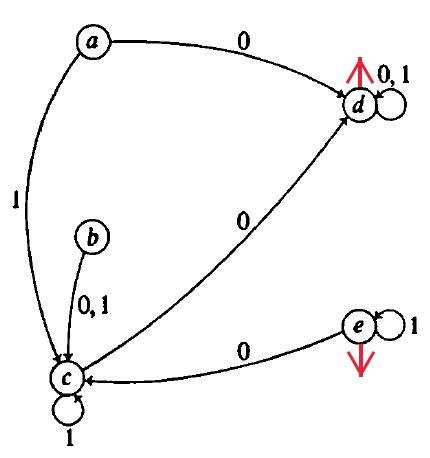
\includegraphics[scale=0.4] {mini-fa} 
	\begin{tikzpicture}[->,>=stealth',shorten >=1pt,auto,node distance=1.5cm, semithick]
	\tikzstyle{every state}=[minimum size=0.1mm]
	\node[state] (a) {$a$};
	\node[state,accepting] (d) [right of=a] {$d$};
	\node[state] (c) [below of=a] {$c$};
	\node[state] (b) [left of=c] {$b$};
	\node[state,accepting] (e) [right of=c] {$e$};
	\path
	(d) edge [loop above] node {$0,1$} (d)
	(c) edge [loop below] node {$1$} (c)
	(e) edge [loop below] node {$1$} (e)
	(a) edge [] node {$0$} (d)
	(a) edge [swap] node {$1$} (c)
	(b) edge [swap] node {$0,1$} (c)
	(e) edge [] node {$0$} (c)
	(c) edge [] node {$0$} (d)
	;
	\end{tikzpicture}
	\caption{Finite state automaton}
	\label{fig:mini-ex2}
\end{figure}

\section{From \cite{Ratnesh95}}

FSM: Finte State Machine

NFSM: Non-deterministic Finite State Machine without $\epsilon-$moves

DFSM: Deterministic Finite State Machine

\begin{definition}[prefix closure of $K$]
	The prefix closure of $K$, denoted $pr(K)\subseteq\Sigma^\ast$, is the language
	\[pr(K):=\{s\in\Sigma^\ast|\exists t\in K:s\le t \}\]
\end{definition}

\begin{example}[Language]\label{ex:language}
	 Consider for example a buffer of capacity one; it has two different states: empty and full. When an \textit{arrival} event occurs in the empty state, then the buffer becomes full; and when a \textit{departure} event occurs in the full state, then the buffer becomes empty. No other state transition can occur in the buffer. Suppose initially the buffer is empty. Then the language of the buffer consists of all possible sequences of the type:
	 $$arrival\cdot departure\cdot arrival\cdot departure \dots,$$
	 where $``\cdot"$ denotes the operation of concatenation.
	 $\hfill\square$
\end{example}

\begin{example}[Generated language]\label{ex:gen_language}
	Consider the buffer of Example \ref{ex:language} Let $a$, $d$ denote the arrival, departure events respectively. Then the generated language of the buffer is $pr((a\cdot d)^\ast)$. Suppose a trace $s\in pr((a\cdot d)^\ast)$ corresponds to completion of a task if and only if its execution results in the empty state of the buffer. Then the marked language of the buffer equals $(a\cdot d)^\ast$.
	$\hfill\square$
\end{example}

\begin{example}[language model]\label{ex:language_model}
	Consider the buffer of Examples \ref{ex:language} and \ref{ex:gen_language} with language	model $[(ad)^\ast,pr((ad)^\ast)]$. The directed graph shown in Figure \ref{fig:DSM} represents a DSM $G:=(X,\Sigma,\alpha,x_0,X_m)$ for the buffer, where $X=\{empty,full\};\Sigma=\{a, d\}; x_0 = empty; X_m = \{empty\};$ and $\alpha(empty, a) = full, \alpha(full, d) = empty$. Note that $\alpha(empty, d)$ and $\alpha(full, a)$ are not defined; hence the transition function is a partial map. (A node in the graph represents a state; a label on a node represents the name of the corresponding state; a directed edge represents a state transition; a label on a directed edge represents the name of the corresponding event; an arrow entering a node represents an initial state; and a circled node represents a marked state.)
	\begin{figure}[htbp]
		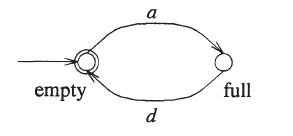
\includegraphics[scale=0.4] {DSM} 
		\caption{Graph representing a DSM}
		\label{fig:DSM}
	\end{figure}
	$\hfill\square$
\end{example}

\begin{example}[Synchronous]
	Consider for example a manufacturing production line consisting
	of a machine (M) and a buffer (B) of capacity one operating in synchrony as shown in Figure \ref{fig:logical-sync}. The event set $\Sigma_1$ of $M$ consists of events $a_1$ representing arrival into the machine, and $d_1$ representing departure from the machine; whereas the event set $\Sigma_2$ of $B$ consists of events $d_1$ representing departure from the machine, and $d_2$ representing departure from buffer. The synchronous composition of two systems is also shown if Figure \ref{fig:logical-sync}.
	\begin{note}
		$d_1$是共享事件,因此,(idle,empty)状态下,$d_1$不能发生, 仅发生 $a_1$事件; (working,empty)状态下,$d_1$在M和B中的转移函数均有定义,因此该共享事件可以发生该共享事件。非共享事件$(a_1,d_2)$在M或B中的转移函数有一个有定义,即可发生。
	\end{note}
	$\hfill\square$
	
	\begin{figure}[htbp]
		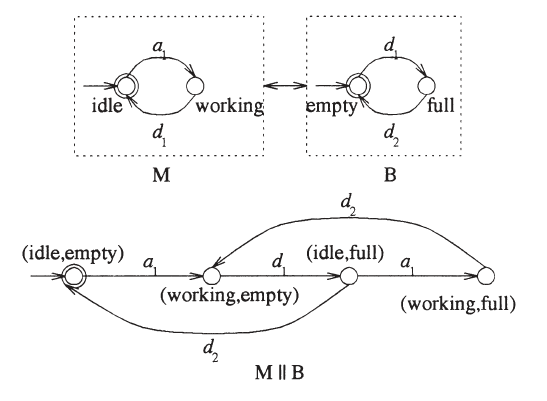
\includegraphics[scale=0.4] {sync} 
		\caption{Diagram illustrating synchronous composition of DFSMs}
		\label{fig:logical-sync}
	\end{figure}
\end{example}

\begin{example}[$\epsilon$-NSM] Consider the $\epsilon$-NSM of Fig. \ref{fig:logical-1model}  Then $\epsilon_G^\ast(1)=\{1,2,3\},\epsilon_G^\ast(2)=\{2,3\},\epsilon_G^\ast(3)=\{3\}.$

so $T(1,\epsilon)=\epsilon_G^\ast(1)=\{1,2,3\}; T(1,a)=\epsilon_G^\ast(T(T(1,\epsilon),a))=\epsilon_G^\ast(T(\{1,2,3\},a)=\epsilon_G^\ast(\{1,3\})=\{1,2,3\}; T(1,ab)=\epsilon_G^\ast(T(\{1,2,3\},b)=\epsilon_G^\ast(\{2\})=\{2,3\}$, etc. $\hfill\square$
	\begin{figure}[htbp]
		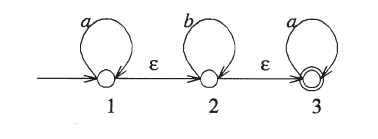
\includegraphics[scale=0.4] {logical-1model} 
		\caption{Diagram illustrating an $\epsilon-NSM$}
		\label{fig:logical-1model}
	\end{figure}
\end{example}


\begin{example}[Completion and reverse]
	Completion and reverse of the DSM of Figure \ref{fig:logical-NFSM-DFSM}(b) are shown
	in Figure \ref{fig:logical-completion-reverse} (a) and \ref{fig:logical-completion-reverse} (b) respectively. The state labels have been changed.
	\begin{figure}[htbp]
		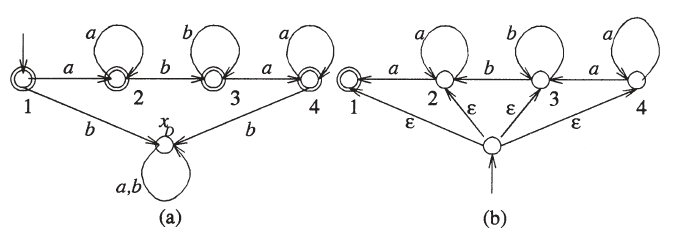
\includegraphics[scale=0.4] {completion-reverse} 
		\caption{Diagram illustrating completion and reverse operations}
		\label{fig:logical-completion-reverse}
	\end{figure}
\end{example}

\begin{theorem}[power set construction]\label{theorem:power_set_cons}
	Let $G:=(X,\Sigma,\alpha,x_0,X_m)$ be a NFSM. Then there exists a language model equivalent DFSM $\mathcal{G}:=(\mathcal{X},\Sigma,\hat{\alpha},\{x_0\},\mathcal{X}_m)$ and $L(\mathcal{G})=L(G)$
\end{theorem}

\begin{proof} Define $\mathcal{X}:=2^X,\mathcal{X}_m:=\{\hat{X}\in\mathcal{X}|\hat{X}\cap X_m\ne \emptyset \}$, and
	\[ \forall \hat{X}\in\mathcal{X},\sigma\in\Sigma:\hat{\alpha}(\hat{X},\sigma):=\bigcup_{x\in\hat{X}}\alpha(x,\sigma) \]
	
	Then is is easily show that $(L_m(\mathcal{G}),L(\mathcal{G}))=(L_m(G),L(G))$
\end{proof}

\begin{example}(NFSM to DFSM)
	Consider the NFSM $G:=(X,\Sigma,\alpha,x_0,X_m)$ shwown in Figure \ref{fig:logical-NFSM-DFSM}(a). The language equivalent DFSM $\mathcal{G}:=(\mathcal{X},\Sigma,\hat{\alpha},\{x_0\},\mathcal{X}_m)$ obtained using the power set construction is shown in Figure \ref{fig:logical-NFSM-DFSM}(b).
	
	Note that $\mathcal{X}=\mathcal{X}_m=\{\{1\},\{1,2,3\},\{2,3\},\{3\} \}$, as $X_m=\{1,3\}$
	
	which has a nonempty intersection with each state in $\mathcal{X}$; 
	\begin{gather*}
	\hat{\alpha}(\{1\},a) = \alpha(1,a) = \{1,2,3\}; \\
	\hat{\alpha}(\{1, 2, 3\}, a) = \alpha(1,a)\cup\alpha(2,a)\cup\alpha(3,a) = \{1, 2, 3\};\\ 
	\hat{\alpha}(\{1, 2, 3\}, b) = \alpha(1, b)\cup\alpha(2, b)\cup\alpha(3, b) = \{2,3\};\\
	etc.
	\end{gather*}

	\begin{figure}[htbp]
		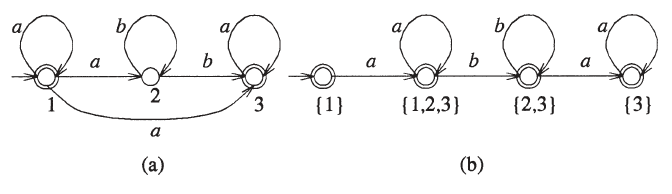
\includegraphics[scale=0.4] {NFSM-DFSM} 
		\caption{Diagram illustrating NFSM to DFSM conversion}
		\label{fig:logical-NFSM-DFSM}
	\end{figure}
\end{example}

\begin{remark}
	It follows from Theorems \ref{theorem:power_set_cons} that if a language model $(K_m, K)$ can be represented as a finite state machine $G$, then there also exists a DFSM $G^\prime$ such that $(L_m(G^\prime), L(G^\prime)) = (K_m, K)$. Thus if we are only concerned with DESs that have finitely many states, then we can assume without loss of generality that they can be represented as DFSMs. We will see below that although the finiteness of states is not needed for most of the analysis, it is needed for developing all the decision algorithms.
	
	However, it should be noted that although DFSMs are useful in developing decision algorithms, it is conceptually easier to obtain a NFSM from the given description of a language. For example, suppose $\Sigma = \{a,b\}$, and suppose we	wish to represent the language with the property that every string in it must contain $aba$ as a substring. A NFSM for the same is shown in Figure \ref{fig:NFSM-DFSM1}(a); corresponding DFSM obtained using the construction outlined in Theorem \ref{theorem:power_set_cons}
	is shown in Figure \ref{fig:NFSM-DFSM1}(b).
\end{remark}

\begin{figure}[htbp]
	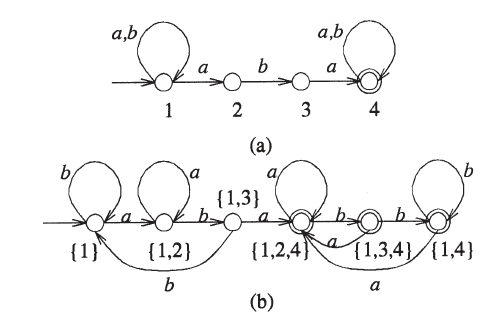
\includegraphics[scale=0.4] {NFSM-DFSM1} 
	\caption{NFSM accepting strings with aba as a substring, and corresponding DFSM}
	\label{fig:NFSM-DFSM1}
\end{figure}

\subsection{Myhill-Nerode Characterization}

\begin{definition}[equivalence relation$(R_K)$]
	Given a language $K\subseteq \Sigma^\ast$, it induces an equivalence relation, denoted $R_K$, on $\Sigma^\ast$:
	\[ \forall s,t\in\Sigma^\ast: s\cong t(R_K)\Leftrightarrow [K\setminus\{s\}=K\setminus\{t\}] \]
	For each $s\in\Sigma^\ast,[s]R_K\subseteq\Sigma^\ast$ is used to denote the equivalence class containing the string $s$.
\end{definition}

\begin{definition}[equivalence relation$(R_G)$]
	Given a DFSM $G:=(X,\Sigma,\alpha,x_0,X_m)$, it induces an equivalence relation, denoted $R_G$, on $\Sigma^\ast$:
	\[ \forall s,t\in\Sigma^\ast: s\cong t(R_G)\Leftrightarrow [\alpha(x_0,s)=\alpha(x_0,t)]\lor[\alpha(x_0,s)=\alpha(x_0,t) \text{ undefined}] \]
	For each $s\in\Sigma^\ast,[s]R_G\subseteq\Sigma^\ast$ is used to denote the equivalence class containing the string $s$.
\end{definition}

\begin{note}
	Note the $R_G$, the \textit{index} of $R_G$, i.e., the number of equivalence classes of $R_G$, is one more than the number of states in $G$, $|R_G|=|G|+1$. (The set of all strings that do not
	belong to $L(G)$ belong to a single equivalence class of $R_G$.) 
\end{note}

It can be easily seen that the equivalence relation $R_G$ refines the equivalence relations $R_{L_m(G)}$ and $R_{L(G)}$. In other words,
\[ \forall s,t\in\Sigma^\ast : s\cong t(R_G)\Rightarrow [s\cong t(R_{L_m(G)})]\land [s\cong t(R_{L(G)})] \]

An equivalence relation $R$ on $\Sigma^\ast$ is said to be \textit{right invariant (with respect to concatenation)} if
\[ \forall s,t\in\Sigma^\ast : s\cong t(R) \Rightarrow su\cong tu(R) \]

It is easy to verify that $R_K$ as well as $R_G$ defined above are right invariant.The following proposition is due to Myhill and Nerode:

\begin{theorem}[Myhill and Nerode]\label{theorem:MyhillNerode}
	Let $K\subseteq\Sigma^ast$ be a language. Then the following are equivalent:
	\begin{enumerate}[1. ]
		\item $K$ is regular.
		\item $K$ can be written as union of some of the equivalence classes of a right invariant equivalence relation of finite index.
		\item $R_K$ is of finite index.
	\end{enumerate}
\end{theorem}

\begin{proof}
	$(1)\Rightarrow (2)$: Suppose $K$ is regular. Then there exists a DFSM $G$ such that $L_m(G) = K$. Then clearly $K$ can be written as union of the following equivalence classes of $R_G$:
	\[\{[s](R_G)|s\in K \}\]
	
	This proves the first assertion implies the second assertion, as $R_G$ is right invariant.
	
	$(2)\Rightarrow (3)$: Let R be a right invariant equivalence relation of finite index such that $K$ can be written as union of some of the equivalence classes of $R$. In order to show that $R_K$ is of finite index it suffices to show that $R$ refines $R_K$. Pick $s,t\in\Sigma^\ast$  such that $s\cong t(R)$. Since $R$ is right invariant, for any $u\in\Sigma^\ast,su\cong tu(R)$. Since $K$ equals union of some of the equivalence classes of $R$, this implies $su\in K$ if and only if $tu\in K$. In other words, $s\cong t(R_K)$, which proves that the second assertion implies the third assertion.
	
	$(3)\Rightarrow (1)$: Finally, suppose $R_K$ is of finite index. Define a DFSM $G:=(\hat{X},\Sigma,\hat{\alpha},\hat{x}_0,\hat{X}_m)$ as follows: $\hat{X}:=\{[s](R_K)|s\in\Sigma^\ast\}; x_0 :=[\epsilon](R_K); \hat{X}_m=\{[s](R_K)|s\in K \}$;
	and
	\[ \forall [s](R_k)\in\hat{X},\sigma\in\Sigma:\hat{\alpha}([s](R_K),\sigma):=[s\sigma](R_K) \]
	
	Then it is readily verified that for each $s\in\Sigma^\ast,\hat{\alpha}(\hat{x}_0,s)=[s](R_K)$. Hence
	from definition of marked language we obtain that $s\in L_m(G)$ if and only if $\hat{\alpha}(\hat{x}_0,s) = [s](R_K) \in X_m$, i.e., if and only if $s\in K$. Thus $L_m(G) = K$. Since $\hat{G}$ is a DFSM (as $R_K$ is of finite index), this implies that $K$ is regular; so the third assertion implies the first assertion. $\hfill\square$
\end{proof}

The construction of the DFSM G in the proof of Theorem \ref{theorem:MyhillNerode} is known as the Myhill-Nerode construction. The following example illustrates such a construction.

\begin{example}[equivalence classes]
	Consider for example the marked language $K_m = (ad)^\ast$ of
	the buffer of capacity one of Example \ref{ex:gen_language}. 
	Then the generated language of the buffer is $pr((a\cdot d)^\ast)=pr(K_m)$. Suppose a trace $s\in pr((a\cdot d)^\ast)$ corresponds to completion of a task if and only if its execution results in the empty state of the buffer. Then the marked language of the buffer equals $(a\cdot d)^\ast$.
	
	Clearly, $K_m$ is a regular language.
	Hence it follows from Theorem \ref{theorem:MyhillNerode} that $R_{K_m}$ is of finite index. It can be easily verified that
	\begin{gather*}
		[\epsilon](R_{K_m})=(ad)^\ast=K_m\\
		[a](R_{K_m})=(ad)^\ast a=pr(K_m)-K_m\\
		[d](R_{K_m})=\{a,d\}^\ast-pr(K_m)
	\end{gather*}
	and these are the only equivalence classes of $R_{K_m}$
	
	Hence Myhill-Nerode construction yields the DFSM $G:=(\hat{X},\Sigma,\hat{\alpha},\hat{x}_0,\hat{X}_m)$, while\\ 
	$\hat{X}=\{[\epsilon](R_{K_m}),[a](R_{K_m}),[d](R_{K_m}) \}$;
	$\hat{x}_0=[\epsilon](R_{K_m}); X_m=\{[\epsilon](R_{K_m}) \}$;\\
	and
	\begin{align*}
		\hat{\alpha}([\epsilon](R_{K_m}),a)&=[a](R_{K_m});\\
		\hat{\alpha}([\epsilon](R_{K_m}),d)&=[d](R_{K_m});\\
		\hat{\alpha}([a](R_{K_m}),a)&=[aa](R_{K_m})=[d](R_{K_m});\\
		\hat{\alpha}([a](R_{K_m}),d)&=[ad](R_{K_m})=[\epsilon](R_{K_m});\\
		\hat{\alpha}([d](R_{K_m}),a)&=[da](R_{K_m})=[d](R_{K_m});\\
		\hat{\alpha}([d](R_{K_m}),d)&=[dd](R_{K_m})=[d](R_{K_m});
	\end{align*}
	
	See figure \ref{fig:equiv}, State e: empty,$[\epsilon](R_{K_m})$;
	State f: full,$[a](R_{K_m})$;  State t: dump/trap,$[d](R_{K_m})$.
	
	\begin{figure}[htbp]
      \centering
	  \subfigure[buffer model]
	  {
	  	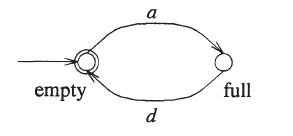
\includegraphics[scale=0.4] {DSM}
	  }
      \hspace{2cm} % 如果并列,用\\换行即可
      \subfigure[equivalence classes]
      {
		  \begin{tikzpicture}[->,>=stealth',shorten >=1pt,auto,node distance=2cm, semithick]
		  \tikzstyle{every state}=[minimum size=0.1mm]
		  \node[state]         (t) {t};
		  \node[initial,state,accepting] (e) [above left of=t] {e};
		  \node[state]         (f) [above right of=t] {f};
		  \path
		  (e) edge [bend left]  node {$a$} (f)
		      edge [swap] node {$d$} (t)
		  (f) edge [bend left]  node {$d$} (e)
		      edge [] node {$a$} (t)
		  ;
		  \end{tikzpicture}
		  (states e:empty,f:full,t:dump/trap) 
      }
	  \caption{equivalence classes}
	  \label{fig:equiv}
	\end{figure}
	$\hfill\square$
\end{example}

\begin{remark}
	Given a regular language K, there always exists a DFSM $G$ such
	that $L_m(G) = K$. Hence there exists a minimal such DFSM (one with a minimal number of states). Let $G^\prime$ be the DFSM obtained by removing the state $[s](R_K)$ form $\hat{G}$ (and all transitions leading into/out of it), where $\hat{G}$ is the DFSM in the proof of Theorem \ref{theorem:MyhillNerode} and $s\in \Sigma^\ast$ is such that $s\notin pr(K)$.Then it is easy to see that $L_m(G^\prime) = K$. In fact $G^\prime$ is a minimal DFSM with marked language $K$. In order to see this first note that the number of states in $\hat{G}$ is $|R_K|$, the index of $R_K$. Since $G^\prime$ is obtained by removing a single state from $\hat{G}$, the number of states in $G^\prime$ equals $|R_K|-1$. Let $G$ be any DFSM with $L_m(G) = K$. Then as noted above number of states in $G$ equals $|R_G|-1$. Also,as noted above, $R_G$ refines $R_{L_m(G)} = R_K$, which implies that $|R_K|\le |R_G|$. Thus $|R_K| - 1\le |R_G| - 1$, which proves that $G^\prime$ is a minimal DFSM with marked language $K$.
\end{remark}

\subsection{Minimization}

\begin{theorem}[Minimal $K$] \label{theorem:Minimal}
	Suppose $K\subseteq \Sigma^\ast$ is a regular language. Then a trim DFSM $G:=(X,\Sigma,\alpha,x_0,X_m)$ with marked language $K$ is mininmal if and only if
	$$\forall x,x^\prime\in X,s\in \Sigma^\ast :(\alpha(x,s),\alpha(x^\prime,s))\in X_m\times X_m\Rightarrow x=x^\prime .$$
\end{theorem}

Suppose $K\subseteq \Sigma^\ast$ is regular. Let $G:=(X,\Sigma,\alpha,x_0,X_m)$ be a trim DSFSM such that $L_m(G)=K$. We are interested in obtaining a minimal DFSM with marked language $K$ by combining some of the ``language equivalent" states of $G$. Note that if $K = \Sigma^\ast$, then it can be accepted by a minimal DFSM having a single state. Hence we assume without loss of generality that $K\ne\Sigma^\ast$.

DFSM $G:=(X,\Sigma,\alpha,x_0,X_m)$ induces an equivalence relation on $X$ defined as:
\[ \forall x,x^\prime\in X:x\cong x^\prime \Leftrightarrow [\forall s\in\Sigma^\ast:\alpha(x,s)\in X_m\Leftrightarrow\alpha(x^\prime,s)\in X_m] \]

Using this equivalence relation we define a language equivalent DFSM $\hat{G}:=(\hat{X},\Sigma,\hat{\alpha},\hat{x}_0,\hat{X}_m)$, where $\hat{X}:=\{[x]|x\in X\},\hat{x}_0:=[x_0],\hat{X}_m:=\{[x]|x\in X_m\}$, and
\[
\forall [x]\in\hat{X},\sigma\in\Sigma:\hat{\alpha}([x],\sigma):=\left\{ 
\begin{aligned}
\left[\alpha(x,\sigma)\right]  &\text{   if $\alpha(x,\sigma)$ defined}\\ 
\text{undefined} &\text{    otherwise}\\
\end{aligned} 
\right. 
\]

Using the fact that $G$ is trim, it is readily verified that $\hat{G}$ is well defined, and $(L_m(\hat{G}),L(\hat{G}))=(L_m(G),L(G))=(K,pr(K))$. Moreover, it follows from Theorem \ref{theorem:Minimal} that $\hat{G}$ is a minimal state machine with marked language $K$.

An algorithm for efficiently identifying the equivalence classes $\{[x]|x\in X\}$ is presented next. Note that each state pair $(x,x^\prime)\in (X_m\times X_m)\cup [(X-X_m)\times (X-X_m)]$ is a possible pair of equivalent states. 

First consider $\bar{G}:=(\bar{X},\Sigma,\bar{\alpha},x_0,X_m)$, the completion of $G$. Then since $K\ne\Sigma^\ast,X_m\ne\bar{X}=X\cup\{x_D\}$, while $X_D$ is the ``dump" state. This implies $\bar{X}-X_m\ne\emptyset$.

\begin{note}
	Note that if $K = \Sigma^\ast$, then it can be accepted by a minimal DFSM having a single state.
\end{note}

\begin{figure}[htbp]
	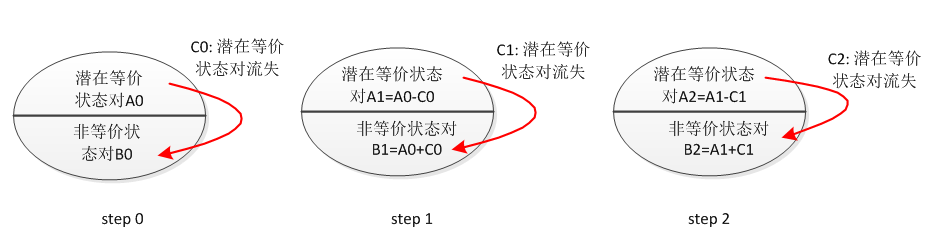
\includegraphics[scale=0.4] {algo-minimize} 
	\caption{Diagram illustrating algorithm minimize}
	\label{fig:algo-minimize}
\end{figure}

\begin{algorithm}  
	\caption{The algorithm for a minimal DFSM, see Figure \ref{fig:algo-minimize}}  
	\begin{algorithmic}[1] %每行显示行号  
		\Require $G=(\bar{X},\Sigma,\alpha,\_,X_m)$  
		\Ensure The equivalence classes of $X$ 
		
		A: \{潜在等价状态对\}; B: \{非等价状态对\}; C: \{本次迭代流失的潜等价状态对\}
		
		\State Initiation step:
		
		$A_0 := [X_m\times X_m]\cup [(\bar{X}-X_m)\times(\bar{X}-X_m)]=\{\text{(final状态对)}\cup \text{(非final状态对)} \} = \{\text{潜在的等价状态对}\}$; 
		
		$B_0 := [\bar{X}\times\bar{X}-A_0] = \{\text{(全体状态对)}-A_0 \} = \{\text{(final状态,非final状态)} \} = \{\text{非等价状态对}\} = \{\text{非$A_0$状态对}\}$; 
		
		$k:=0$.
		
		\State Iteration step:
		\begin{align*}
			C_k &:= \{(x,x^\prime)\in A_k | \exists\sigma\in\Sigma \text{ s.t. } (\alpha(x,\sigma),\alpha(x^\prime,\sigma))\in B_k \} \\
			&=\{\text{$A_0$中两大类中的(状态对)存在字母$\sigma$进入$B_0$类)} \} \\
			&= \{ \text{潜在状态对 $\to$ 非等价状态对} \}\\
			A_{k+1} &:= A_k - C_k \\
			B_{k+1} &:= B_k\cup C_k =[\bar{X}\times \bar{X}] - A_{k+1}\\
			&=\{\text{非$A_{k+1}$状态对}\}
		\end{align*}
		
		\State Termination step:
		
		if $A_{k+1}=A_k$, then stop; else, $k := k+1$, and goto step 2.
	\end{algorithmic}
    \label{alg:minimal}   
\end{algorithm}

It can be verified that after termination, each state pair in $A_k$ is an equivalent pair of states. Finally, the minimal state machine $G$ is obtained by combining each state pair in $A_k$ as described above, and removing the equivalence class of the dump state.

Algorithm \ref{alg:minimal} terminates in $O(m^2)$ steps, where $m$ is the number of states in $G$.

\begin{example}
	Consider the complete DFSM of Figure \ref{fig:complete}. Then $X_m=\{1,2,3,4 \}$ and $X=\{1,2,3,4,x_D \}$. Algorithm \ref{alg:minimal} can be  applied to minimize the DFSM as follows:
	\begin{align*}
		A_0 &=[X_m\times X_m]\cup\{(x_D\times x_D)\};\\
		&=\{(1,1),(2,2),(3,3),(4,4),(1,2),(2,1),(1,3),(3,1),(1,4),(4,1),(2,3),(3,2),(2,4),(4,2),(3,4),(4,3) \} \cup\{(x_D,x_D) \}\\
		&=\{(1,1),(2,2),(3,3),(4,4) \}\cup\{(1,2),(1,3),(1,4),(2,3),(2,4),(3,4) \}\cup
		\{(2,1),(3,1),(4,1),(3,2),(4,2),(4,3)\}\cup\{x_D,x_D\}\\
		&= \{\text{潜在的等价状态对}\} \\
		B_0 &=[X\times X]-A_0\\
		&=\{(1,x_D),(x_D,1),(2,x_D),(x_D,2),(3,x_D),(x_D,3),(4,x_D),(x_D,4) \}\\
		&=\{(1,x_D),(2,x_D),(3,x_D),(4,x_D) \} \cup \{(x_D,1),(x_D,2),(x_D,3),(x_D,4) \}\\
		&= \{\text{非等价状态对}\} = \{\text{非$A_0$状态对}\}\\
		C_0 &= \{(1,2),(2,1),(1,3),(3,1),(2,4),(4,2),(3,4),(4,3)\}\\
		&=\{(1,2),(1,3),(2,4),(3,4) \}\cup\{(2,1),(3,1),(4,2),(4,3) \}\\
		&= \{ \text{潜在状态对$(A_0) \to (B_0)$非等价状态对} \}\\
		A_1 &= A_0-C_0\\
		&=\{(1,1),(2,2),(3,3),(4,4) \}\cup\{(1,4),(2,3) \}\cup
		\{(4,1),(3,2) \}\cup\{x_D,x_D\}\\
		B_1 &= [X\times X]-A_1\\
		&= \{\text{非$A_1$状态对}\}\\
		C_1 &= \{ \text{潜在状态对($A_1) \to (B_1)$非等价状态对} \}\\
		&= \{(1,4),(4,1),(2,3),(3,2)\}\\
		A_2 &= A_1-C_1\\
		&= \{(1,1),(2,2),(3,3),(4,4),(x_D,x_D)\}\\
		B_2 &=[X\times X] - A_2
	\end{align*}
    Clearly, all the state pairs in $A_2$ are equivalent pairs, i.e. $C_2 = \emptyset$: hence the algorithm terminates. Thus the minimal DFSM is the DFSM of Figure \ref{fig:complete}, which does not contain the dump state.
	\begin{figure}[htbp]
		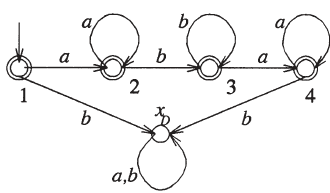
\includegraphics[scale=0.4] {complete} 
		\caption{the minimal DFSM is not contain the dump state}
		\label{fig:complete}
	\end{figure}
\end{example}

\section{From \cite{Jean2011}}

\begin{definition} [Partitions and equivalence relations]
	A partition of a set $E$ is a family $P$ of nonempty,	pairwise disjoint subsets of $E$ such that $E =	\bigcup_{\mathcal{P}\in P}\mathcal{P}$. The \textit{index} of the partition is the number of its elements. A partition defines an equivalence relation $\equiv p$ on $E$. Conversely,
	the set of all equivalence classes $[x]$, for $x \in E$, of an equivalence relation on $E$ defines	a partition of $E$. This is the reason why all terms defined for partitions have the same
	meaning for equivalence relations and vice versa.
\end{definition}

A subset $F$ of $E$ is \textit{saturated}使充满 by $P$ if it is the union of classes of $P$. Let $Q$ be another partition of $E$. Then $Q$ is a \textit{refinement} of $P$, or $P$ is \textit{coarser} than $Q$, if each class of $Q$ is contained in some class of $P$. If this holds, we write $Q \le P$. The index of $Q$ is then larger than the index of $P$.

Given two partitions $P$ and $Q$ of a set $E$, we denote by $U = P\land Q $ the coarsest partition粗划分 which refines $P$ and $Q$. The classes of $U$ are the nonempty sets $\mathcal{P}\cap \mathcal{Q}$, for $\mathcal{P} \in P $ and $\mathcal{Q} \in Q.$ The notation is extended to a set of partitions in the usual way: we write $P = P_1\land\cdots P_n$ for the common refinement of $P_1,\dots,P_n$. If $n = 0$, then $P$ is
the universal partition of $E$ composed of the single class $E$. This partition is the neutral element for the $\land$-operation.

Let $F$ be a subset of $E$. A partition $P$ of $E$ induces a partition $P^\prime$ of $F$ by intersection: $P^\prime$ is composed of the nonempty sets $\mathcal{P}\cap F$, for $\mathcal{P}\in P$ If $P$ and $Q$ are partitions of $E$
and $Q\le P$, then the restrictions $P^\prime$ and $Q^\prime$ to $F$ still satisfy $Q^\prime \le P^\prime$.

If $P$ and $P^\prime$ are partitions of disjoint sets $E$ and $E^\prime$, we denote by $P\lor P^\prime$ the partition
of $E\cup E^\prime$ whose restriction to $E$ and $E^\prime$ are $P$ and $P^\prime$ respectively. So, one may write
\[ P =\bigvee_{\mathcal{P}\in P}\{\mathcal{P}\} \]

\begin{definition}[Minimal automaton]
	We consider a deterministic automaton $A = (Q, i, F)$ over the
	alphabet $A$ with set of states $Q$, initial state $i$, and set of final states $F$. To each state $q$ corresponds a subautomaton of $A$ obtained when $q$ is chosen as the initial state. We call it the \textit{subautomaton rooted at $q$} or simply the automaton at $q$. Usually, we consider only	the trim part of this automaton. To each state q corresponds a language $L_q(A)$ which is the set of words recognized by the subautomaton rooted at q, that is
	\[L_q(A)=\{w\in A^\ast |q\cdot w\in F\} \]
	
	This language is called the \textit{future} of the state $q$, or also the \textit{right language} of this state. Similarly one defines the \textit{past} of $q$, also called the \textit{left language}, as the set $\{w\in A^\ast|i\cdot w = q \}$. The automaton $A$ is \textit{minimal} if $L_p(A) \ne Lq(A)$ for each pair of distinct states $p, q$. The equivalence relation $\equiv$ defined by
	\[p\equiv q \text{ if and only if } L_p(A)=L_q(A) \]
	is a \textit{congruence}, that is $p\equiv q$ implies $p\cdot a ≡ q\cdot a$ for all letters $a$. It is called the \textit{Nerode congruence}. Note that the Nerode congruence saturates the set of final states. Thus an	automaton is minimal if and only if its Nerode equivalence is the identity.
\end{definition}

Minimizing an automaton is the problem of computing the Nerode equivalence. Indeed, the $quotient$ automaton $A/\equiv$ obtained by taking for set of states the set of equivalence classes of the Nerode equivalence, for the initial state the class of the initial state $i$, for set of final states the set of equivalence classes of states in $F$ and by defining the transition function by $[p]\cdot a = [p\cdot a]$ accepts the same language, and its Nerode equivalence is the identity. The minimal automaton recognizing a given language is unique.

\begin{definition} [Partitions and automata]
	Again, we fix a deterministic automaton $A = (Q, i, F)$ over
	the alphabet $A$. It is convenient to use the shorthand $P^c$ for $Q\setminus P$ when $P$ is a subset of the set $Q$.
	
	Given a set $P\subset Q$ of states and a letter $a$, we denote by $a^{-1}P$ the set of states $q$ such	that $q\cdot a\in P$.  Given sets $P,R\subset Q $ and $a\in A$, we denote by
	\[(P,a)|R\]
	the partition of $R$ composed of the nonempty sets among the two sets
	\[R\cap a^{-1}P=\{q\in R|q\cdot a\in P\} \text{ and } R\setminus a^{-1}P =\{q\in R|q\cdot a\notin P \} \]
	Note that $R\setminus a^{-1}P=R\cap(a^{-1}P)^c=R\cap a^{-1}(P^c)$ so the definition is symmetric in $P$ and $P^c$. In particular
	\begin{align}
	  (P,a)|R=(P^c,a)|R %\label{key1}
	\end{align}
	
\end{definition}

%%%%%%%%%%%%%%%%%%%%%%%%%%%%%%%%%%%%%%%%%%%%%%%%%%5
\begin{thebibliography}{99}
	\bibitem[Hopcroft71]{Hopcroft71}
	Hopcroft, J.E. \textit{An n log n algorithm for minimizing states in a finite automaton}, in The Theory of Machines and Computations (Z. Kohavi, ed.), pp.180-196, Academic Press, New York, 1971.
	
	\bibitem[Gries73]{Gries73}
	Gries, D. \textit{Describing an Algorith m by Hopcroft}, Acta Inf. 2:97 109, 173. $\copyright$ by Springer-Verlag 1973
	
	\bibitem[Ratnesh95]{Ratnesh95}
	Ratnesh Kumar, \textit{Modeling and Control of Logical Discrete Event Systems}, $\copyright$ 1995 by Springer Science+Business Media New York.
	
	\bibitem[Jean2011]{Jean2011}
	Jean Berstel, Luc Boasson, Olivier Carton, Isabelle Fagnot
	, \textit{Minimization of automata}, Universit$\acute{e}$ Paris-Est Marne-la-Vall$\acute{e}$e 2010 Mathematics Subject Classification: 68Q45, 2011.
	
\end{thebibliography}
